\documentclass[usenames,dvipsnames,t]{beamer}
\usepackage[english]{babel}
\usepackage[utf8]{inputenc}
\usepackage{amsmath,amsthm, amssymb, latexsym}
\usepackage{color}
\usepackage{tikz}
\usepackage{standalone}
\usepackage{minted}
\usepackage{hyperref}
\usepackage{graphicx}
\usepackage{wrapfig}
\usepackage{rotating}
\usepackage{fontawesome}
\usepackage{multicol}
\usepackage{enumitem}
\setitemize{label=\usebeamerfont*{itemize item}%
  \usebeamercolor[fg]{itemize item}
  \usebeamertemplate{itemize item}}

\usepackage[utf8]{inputenc}
\DeclareUnicodeCharacter{2010}{-}% support older LaTeX versions

\makeatletter
\setlength{\@fptop}{0pt}
\makeatother
\setlength{\columnsep}{2pt}

\definecolor{DarkGray}{RGB}{7, 54, 66}
\usemintedstyle{native}

\usetikzlibrary{decorations.pathmorphing}
\usetikzlibrary{fit}                    % fitting shapes to coordinates
\usetikzlibrary{backgrounds}    % drawing the background after the foreground
\usetikzlibrary{arrows}
\usetikzlibrary{decorations.markings}

\tikzstyle{background}=[red!79, rectangle, draw, inner sep=-0.5mm,
           rounded corners=1mm, thick]

\usecolortheme[dark,accent=cyan]{solarized}
\beamertemplatenavigationsymbolsempty
\setbeamerfont{block title}{size=\Large}
\usepackage[orientation=landscape,size=a0,scale=1.4]{beamerposter}

%%%%%%%%%%%%%%%%%%%%%%%%%%%%%%%%%%%%%%%%%%%%%%%%%%%%%%%%%%%%%%%%%%%%%%%%%%%%%%%
\begin{document}
\begin{frame}[fragile]

%%%%%%%%%%%%%%TOP ROW%%%%%%%%%%%%%%%%%%
\begin{columns}
  \begin{column}{.49\linewidth}
   \vspace{1cm}

    \centering
    {\fontsize{120}{130}\selectfont\textcolor{orange}{PIP \hspace{2cm} INSTALL \hspace{2cm} AXELROD}}
    % \large{THE \textcolor{brown}{ITERATED PRISONERS DILEMMA}
    % ALLOWS THE STUDY OF \textcolor{brown}{COOPERATIVE BEHAVIOUR}}
    \Large{
    \begin{multicols}{2}
    \begin{itemize}
      \item both sides are better off \textbf{Cooperating} (3)
      \item but there is always a tempetation to \textbf{Defect} (5)
    \end{itemize}
    \end{multicols}
    }
  \end{column}
  \begin{column}{.25\linewidth}

    \centering
   \includestandalone[width=0.65\textwidth]{static/matrix}
  \end{column}
  % \begin{column}{.35\linewidth}

  %   \large{
  %   AXELROD LIBRARY IS AN OPEN SOURCE TOOL THAT COMBINES
  %   \textcolor{cyan}{PYTHON} \textbf{+} \textcolor{brown}{PRISONERS DILEMMA}}
  %   \large{
  %   \begin{itemize}%[leftmargin=1.7in]
  %   \item more than \textcolor{brown}{200 condtibutors}
  %   \item \textcolor{brown}{100\%} test coverage
  %   \item unit and integration \textcolor{brown}{tests}
  %   \item \textcolor{brown}{documentation}.
  %   \end{itemize}
  %   }
  % \end{column}
%   \begin{column}{.10\linewidth}

  \end{columns}
  \begin{columns}
    \begin{column}{.25\linewidth}
%%%%%%%%%%%%%%%%%%FIRST QUESTION%%%%%%%%%%%%%%%%%% 
   \vspace{1cm}

\begin{center}
\Large{\textcolor{red!80}{WHEN INTERACTING WITH A SNEAKY OPPONENT}}
\end{center}
\begin{center}
\Large{\textcolor{red!80}{SHOULD PEOPLE HOLD A GRUDGE AGAINST THEM?}}
\end{center}

\vspace{1cm}

\noindent\rule[0.5ex]{\linewidth}{1pt}

\begin{figure}
\begin{center}
\includestandalone[width=0.9\textwidth]{static/match}
\end{center}
\end{figure}

\vspace{0.5cm}

    \begin{minted}
    [
    autogobble=true,       
    frame=lines,
    framesep=2mm,
    fontsize=\normalsize,
     bgcolor=DarkGray,  
    ]
    {python}

>>> import axelrod as axl

>>> first_match = axl.Match([
        axl.SneakyTitForTat(), 
        axl.Grudger()], turns=100)

>>> first_match.play()[:6]
[('C', 'C'), ('C', 'C'), ('D', 'C'), 
 ('D', 'D'), ('C', 'D'), ('C', 'D')]

>>> print(first_match.sparklines())             

>>> first_match.final_score()
(295, 60)

>>> second_match = axl.Match([
        axl.SneakyTitForTat(), 
        axl.TitForTat()], turns=100)

>>> second_match.play()
>>> second_match.final_score()
(297, 297)
\end{minted}
    \end{column}
    \begin{column}{.25\linewidth}
%%%%%%%%%%%%%%%%%SECOND QUESTION%%%%%%%%%%%%%%%%%% 
   \vspace{1cm}
   
\begin{center}
    \Large{\textcolor{OliveGreen}{WHAT THE OPTIMAL STRATEGIC PLAY AGAINST THE MANY FACES OF WAR?}} 
    \end{center}

\vspace{3.5cm}

\centering
\includestandalone[width=\textwidth, height=0.3\textwidth]{static/tournament}

\vspace{2cm}

    \begin{minted}
    [
    autogobble=true,          
    frame=lines,
    framesep=2mm,
    fontsize=\normalsize,
    bgcolor=DarkGray,  
    ]
    {python}
>>> import axelrod as axl

>>> axl.seed(0)
>>> players = [axl.Cooperator(), axl.Random(), 
               axl.TitForTat(), axl.Grudger(), 
               axl.Defector()]

>>> tournament = axl.Tournament(players)
>>> results = tournament.play()
>>> results.ranked_names
['Defector', 'Grudger', 'Tit For Tat', 
 'Cooperator', 'Random: 0.5']

>>> plot = axl.Plot(results)
>>> p = plot.boxplot()
>>> p.show()
\end{minted}

    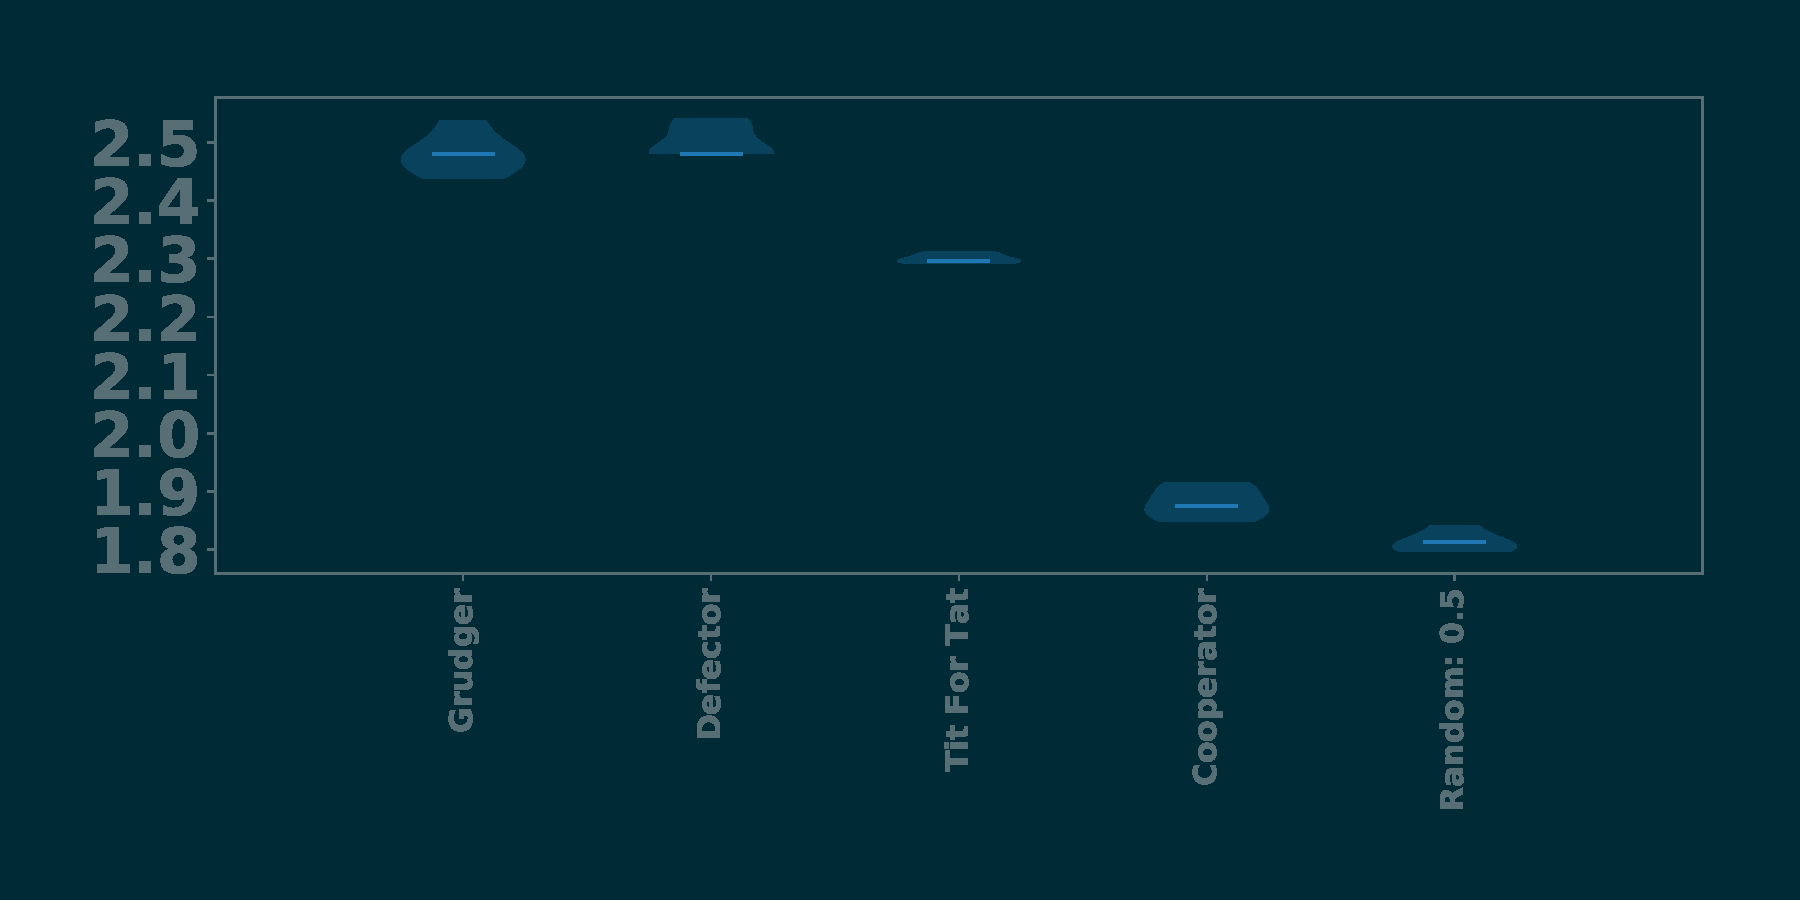
\includegraphics[width=\textwidth, height=0.65\textwidth]{static/tournament_results.pdf}
  \end{column}
      \begin{column}{.25\linewidth}
%%%%%%%%%%%%%%%%%%THIRD QUESTION%%%%%%%%%%%%%%%%%% 
   \vspace{1cm}
   
\begin{center}
        \Large{\textcolor{cyan}{SHOULD THE NORTH JOIN HANDS WITH THE SOUTH TO DEFEAT THE NIGHT KING?}} 
\end{center}

   \vspace{0.3cm}

        \begin{center}
        \includestandalone[width=1.05\textwidth]{static/evolution}
        \end{center}
    \begin{center}

    \begin{minted}
    [
    autogobble=true,          
    frame=lines,
    framesep=2mm,
    fontsize=\small,
    bgcolor=DarkGray,
    ]
    {python}
>>> import random

>>> N = 5
>>> players = []
>>> axl.seed(5)
>>> for _ in range(N):
    ... player = random.choice([axl.Defector, 
                                axl.Cooperator])
    ... players.append(player())
    
>>> mp = axl.MoranProcess(players=players, turns=200)
>>> mp.play()

[Counter({'Cooperator': 3, 'Defector': 2}),
 Counter({'Cooperator': 3, 'Defector': 2}),
 Counter({'Cooperator': 3, 'Defector': 2}),
 Counter({'Cooperator': 2, 'Defector': 3}),
 Counter({'Cooperator': 2, 'Defector': 3}),
 Counter({'Cooperator': 1, 'Defector': 4}),
 Counter({'Cooperator': 1, 'Defector': 4}),
 Counter({'Cooperator': 1, 'Defector': 4}),
 Counter({'Defector': 5})]
    \end{minted}

   \vspace{1cm}

    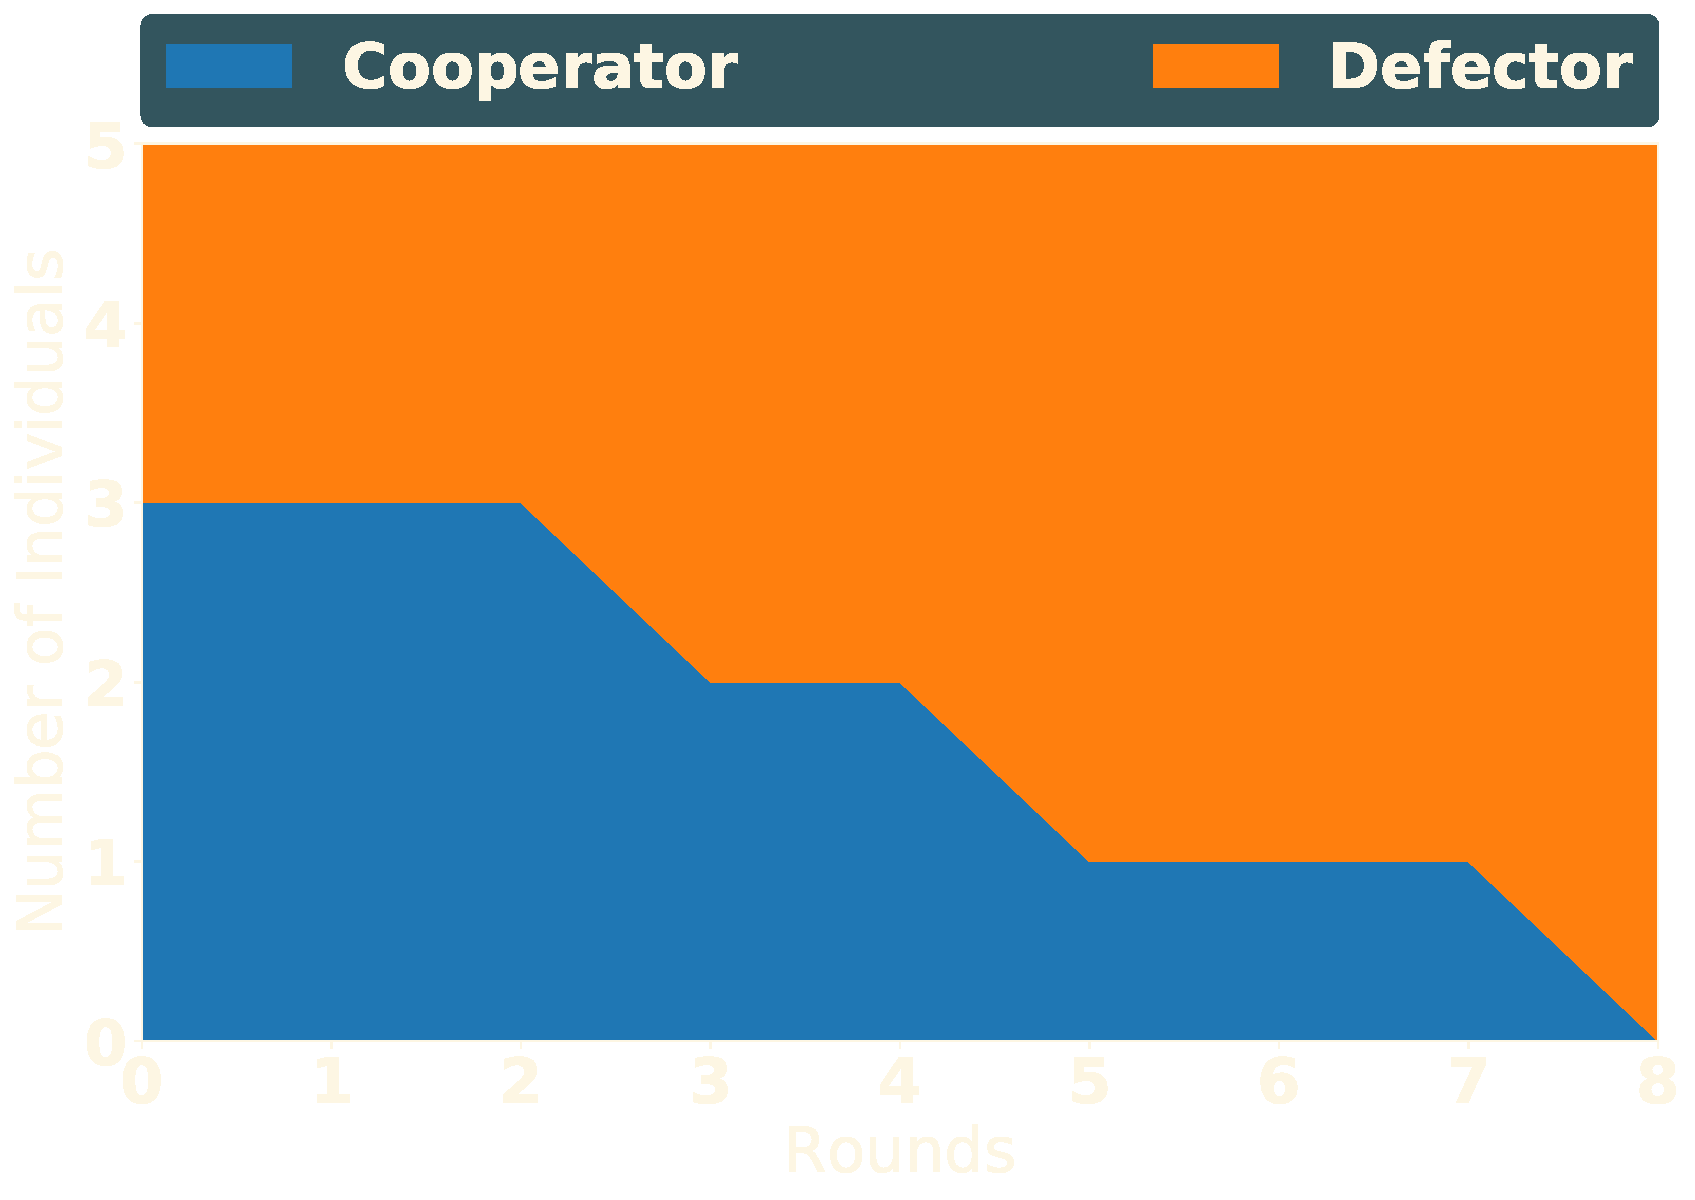
\includegraphics[width=0.7\textwidth, height=0.5\textwidth]{static/evolution_results.pdf}
    \end{center}

    \end{column}
    \end{columns}
\begin{columns}
\begin{column}{.10\linewidth}
\end{column}

\begin{column}{.4\linewidth}

\textbf{
\begin{multicols}{2}
 \begin{itemize}
          \item In case you missed me:
          \item Github: \url{github.com/Axelrod-Python} 
\end{itemize}
\end{multicols}
}
\end{column}
\begin{column}{.2\linewidth}

\textbf{
\begin{multicols}{2}
 \begin{itemize} 
          \item \faTwitter \ NikoletaGlyn 
          \item  \faGithub \ Nikoleta-v 
\end{itemize}
\end{multicols}
}
\end{column}
\end{columns}

   \vspace{1cm}

\end{frame}
\end{document}
% \noindent\rule[0.5ex]{\linewidth}{1pt}

%          

% \hspace{2cm}

% \textbf{ABOUT ME} \\

% \begin{itemize}
% \item[] \hspace{-1.2cm} \faTwitter \ NikoletaGlyn \ \faGithub \ Nikoleta-v3
% \end{itemize}
% }